\section{Deep Learning 1}\label{deep-learning-1}

\subsection{Classical CV Pipeline}\label{classical-cv-pipeline}

\subsubsection{Pipeline}\label{pipeline}

\begin{enumerate}
  \def\labelenumi{\arabic{enumi}.}
  \item
        \textbf{Keypoint detector}

        关键点检测器，找到图像中有意义的点（角点、斑点等）。 例如 Harris
        corner detector。
  \item
        \textbf{Keypoint descriptor}

        关键点描述子，在兴趣点周围提取局部特征向量。 例如 SIFT。
  \item
        \textbf{Image representation}

        图像表示，把多局部特征聚合成固定长度向量（如直方图），便于分类器处理。
        例如 Bag-of-Visual-Words。
  \item
        \textbf{Classifier}

        分类器，在聚合表示上训练浅模型完成最终分类任务。 例如 SVM, logistic
        regression
\end{enumerate}

\subsubsection{Keypoint detector}\label{keypoint-detector}

Where to
look。传统算法多基于梯度、Hessian、角点响应等设计启发式准则。常见的方法有
Harris，DoG 等。

\subsubsection{Descriptor}\label{descriptor}

What is around that point。常见的方法有 \textbf{SIFT（Scale-Invariant
  Feature Transform）}，配合 DoG 使用可以做到尺度等变性。

SIFT 的步骤：

本质上是把每个关键点映射成一个定长的特征向量，且这种映射具有鲁棒性。

\begin{enumerate}
  \def\labelenumi{\arabic{enumi}.}
  \tightlist
  \item
        检测出\textbf{关键点}。
  \item
        为每个关键点确定\textbf{主方向}（orientation），通常使用圆形邻域进行
        vote（注意需要按距离加权）。并做方向归一化，也即进行旋转使主方向朝向
        \(0 \circ\)。
  \item
        旋转后，在关键点周围选取一个 \(16 \times 16\) 的
        \textbf{patch}，注意坐标不一定整数，需用双线性插值。
  \item
        将该 patch 划分为 \(4 \times 4\) 个子区域，每子区域 \(4 \times 4\)
        像素。 把 \(360 \circ\) 分成 \(8\) 个
        bins，每个子区域像素以梯度大小为权加入 bins，最后每个子区域得到一个
        \textbf{\(8\) 维向量}。
  \item
        合起来得到 \(128\)
        维描述子，最后进行归一化、阈值截断、再归一化。其中归一化是避免整体亮度变化影响，阈值截断是避免局部阴影的影响。
\end{enumerate}

\subsubsection{Aggregation}\label{aggregation}

How the whole image is。常见的方法有 \textbf{Bag-of-Visual-Words}。

BoVW 的步骤：

本质上是把不确定数量的局部描述子映射成固定长度的全局表示。

\begin{enumerate}
  \def\labelenumi{\arabic{enumi}.}
  \tightlist
  \item
        收集\textbf{描述子}。
  \item
        使用聚类算法（如 \textbf{k-means}）把描述子聚成 \(K\) 个簇中心，称为
        \textbf{visual words}。
  \item
        对一张图中每个描述子找最近的 visual
        word，可以是\textbf{硬分配}（单独分配）或\textbf{软分配}（分配权重）。
  \item
        统计每个词的出现次数，得到长度为 \(K\) 的全局表示向量。
\end{enumerate}

\textbf{注}：BoVW
统计词频，不记录词出现的相对位置，故会丢失空间信息。比如鼻子长在眼睛上，BoVW
并不能发现差异。

\subsubsection{Classifier}\label{classifier}

Decision for the task。常用浅学习模型，如 \textbf{logistic
  regression}（二分类）、\textbf{SVM}、小型神经网络等。
本质上是把聚合好的向量映射到类别概率或类别标签。

\textbf{注}：这些分类器只看聚合后的全局表示，不直接访问原像素。

\subsubsection{Problems}\label{problems}

\begin{itemize}
  \tightlist
  \item
        依赖人工设计的特征和启发式规则。
  \item
        流水线会产生错误累积。
  \item
        难以理解高层语义，比如部分（part）、种类（category）、语境（context）等。
  \item
        难以利用海量数据进行优化
  \item
        对某一事物的识别不易泛化到另外事物。
\end{itemize}

\begin{center}\rule{0.5\linewidth}{0.5pt}\end{center}

\subsection{Learning-based CV}\label{learning-based-cv}

\subsubsection{Advantages}\label{advantages}

传统 CV 是设计特征，学习型 CV 是从数据中学习特征。

\textbf{好处}：

\begin{itemize}
  \tightlist
  \item
        \textbf{端到端（end-to-end）}，能直接针对最终任务优化所有参数，避免手工设计中各阶段不一致的目标。
  \item
        自动学习高层语义，从边缘到部分再到对象/场景。
  \item
        能够随数据规模增长而提高性能。
\end{itemize}

\textbf{注}：学习型方法虽然在很多视觉任务中表现更好，但在数据稀缺或\textbf{实时/嵌入式场景}中经典方法仍有价值。

\subsubsection{Why It Took Off}\label{why-it-took-off}

\begin{itemize}
  \tightlist
  \item
        算法（\textbf{Algorithm}）：深度学习架构（多层神经网络、反向传播、优化方法）与研究突破（如
        ReLU、BatchNorm、ResNet 等）。
  \item
        数据（\textbf{Data}）：ImageNet
        等大规模标注数据集让复杂模型能被充分训练。
  \item
        计算资源（\textbf{Compute}）：GPU、TPU
        等硬件加速以及高效并行使大模型训练成为可能。当然电能也非常重要。
\end{itemize}

\begin{center}\rule{0.5\linewidth}{0.5pt}\end{center}

\subsection{Machine Learning}\label{machine-learning}

\subsubsection{Set Up the Task}\label{set-up-the-task}

假设我们想要实现 MNIST
二分类，也即给定一张手写数字图像，判断它是否为数字 5。

输入：\(x \in \mathbb{R}^{784}\)，表示 \(28 \times 28\) 灰度图像展平的
\(784\) 维向量。

标签：\(y \in \{0,1\}\)，是否为数字 5 的标签。

输出：

\begin{itemize}
  \tightlist
  \item
        软分类：\(p(y = 1 | x) \in [0, 1]\)
  \item
        硬分类：\(p(y=1|x) \ge \tau\)，则预测为 1，否则为 0。
\end{itemize}

模型：\(h(x; \theta)\)，其中 \(\theta\) 为待优化参数。

\subsubsection{Prepare the Data}\label{prepare-the-data}

使用 \textbf{MNIST} 数据集。

\textbf{预处理}：

\begin{enumerate}
  \def\labelenumi{\arabic{enumi}.}
  \tightlist
  \item
        标准化：

        \begin{itemize}
          \tightlist
          \item
                将像素值除 \(255\) 从 \([0,255]\) 缩放到 \([0,1]\)。
          \item
                或做零均值单位方差标准化 \(x' = \frac{x-\mu}{\sigma}\)。
        \end{itemize}
  \item
        数据增强：随机平移、旋转少量角度、缩放、弹性变形等。
  \item
        转换为模型需要的数据结构：

        \begin{itemize}
          \tightlist
          \item
                对于线性模型/MLP：展平为 (784,) 向量。
          \item
                对于 CNN：保留形状 (1, 28, 28) 。
        \end{itemize}
  \item
        划分数据集：

        \begin{itemize}
          \tightlist
          \item
                划分为\textbf{训练集}、\textbf{验证集}和\textbf{测试集}。
          \item
                按照训练方法进一步划分，比如划分出 mini-batch。
        \end{itemize}
\end{enumerate}

\textbf{注}：区分 train、validation、test、inference

阶段 \textbar{} 核心目的 \textbar{} 是否更新模型参数 \textbar{}
是否需要标签 \textbar{}\\
:--- \textbar{} :--- \textbar{} :--- \textbar{} :--- \textbar{}\\
\textbf{训练 (Train)} \textbar{} 学习规律 \textbar{} Y \textbar{} Y
\textbar{}\\
\textbf{验证 (Validation)} \textbar{} 调超参数、选模型 \textbar{} N
\textbar{} Y \textbar{}\\
\textbf{测试 (Test)} \textbar{} 最终评估泛化能力 \textbar{} N \textbar{}
Y \textbar{}\\
\textbf{推理 (Inference)} \textbar{} 实际应用预测 \textbar{} N
\textbar{} N \textbar{}

\subsubsection{Build a Model}\label{build-a-model}

模型负责利用给定的输入产生输出，也即给出一个函数
\(h(x; \theta) \in [0, 1]\)，其中 \(\theta\) 为待优化参数。

\paragraph{Logistic Regression}\label{logistic-regression}

逻辑回归，线性模型。

令 \(z = \theta^\top x + b\) 为输入的线性打分。则模型为： \[
  h(x; \theta, b) = \sigma(z) = \frac{1}{1+e^{-z}}
\] 其中参数 \(\theta \in \mathbb{R}^{784}\)，\(b\in\mathbb{R}\)。

\paragraph{MLP Neural Network}\label{mlp-neural-network}

多层感知器（MLP），非线性模型，可以处理非线性可分问题。

若干\textbf{线性层}（矩阵乘法）与\textbf{非线性激活函数}交替堆叠。

每层 \(h = g(Wx + b)\)，其中 \(g\) 是激活函数。

通过施加多层\textbf{非线性变换}， MLP
可以把原来\textbf{线性不可分}的点集映射到一个新的特征空间中，使其\textbf{更线性可分}。

设网络共有 \(L\) 层（含输入输出层）。记：

\begin{itemize}
  \tightlist
  \item
        输入：\(\mathbf{x} \in \mathbb{R}^{n_1}\)
  \item
        第 \(\ell\) 层的神经元数：\(n_\ell\)
  \item
        第 \(\ell\) 层的权重矩阵：
        \(\mathbf{W}^{(\ell)} \in \mathbb{R}^{n_\ell \times n_{\ell-1}}\)，
        \(w_{ij}^{(\ell)}\) 元代表边
        \(a_j^{(\ell)} \rightarrow a_i^{(\ell+1)}\) 的权重
  \item
        第 \(\ell\)
        层的偏置向量：\(\mathbf{b}^{(\ell)} \in \mathbb{R}^{n_\ell}\)
\end{itemize}

其中 \(\ell = 1, 2, \ldots, L\)。

\textbf{前向传播递推关系}：

\[
  \mathbf{z}^{(\ell)} = \mathbf{W}^{(\ell)} \mathbf{a}^{(\ell-1)} + \mathbf{b}^{(\ell)}, \quad \ell = 1, 2, \ldots, L
\] \[
  \mathbf{a}^{(\ell)} = g_\ell(\mathbf{z}^{(\ell)})
\]

其中：

\begin{itemize}
  \tightlist
  \item
        \(\mathbf{a}^{(1)} = \mathbf{x}\)
  \item
        \(\mathbf{a}^{(\ell)}\) 为第 \(\ell\) 层输出，第 \(\ell + 1\)
        层输入，\(\ell = 1, 2, \ldots, L-1\)
  \item
        \(\mathbf{a}^{(L)}\) 为最终输出
  \item
        \(g_\ell: \mathbb{R}^{n_\ell} \to \mathbb{R}^{n_\ell}\)
        是逐元素激活函数
\end{itemize}

\centering
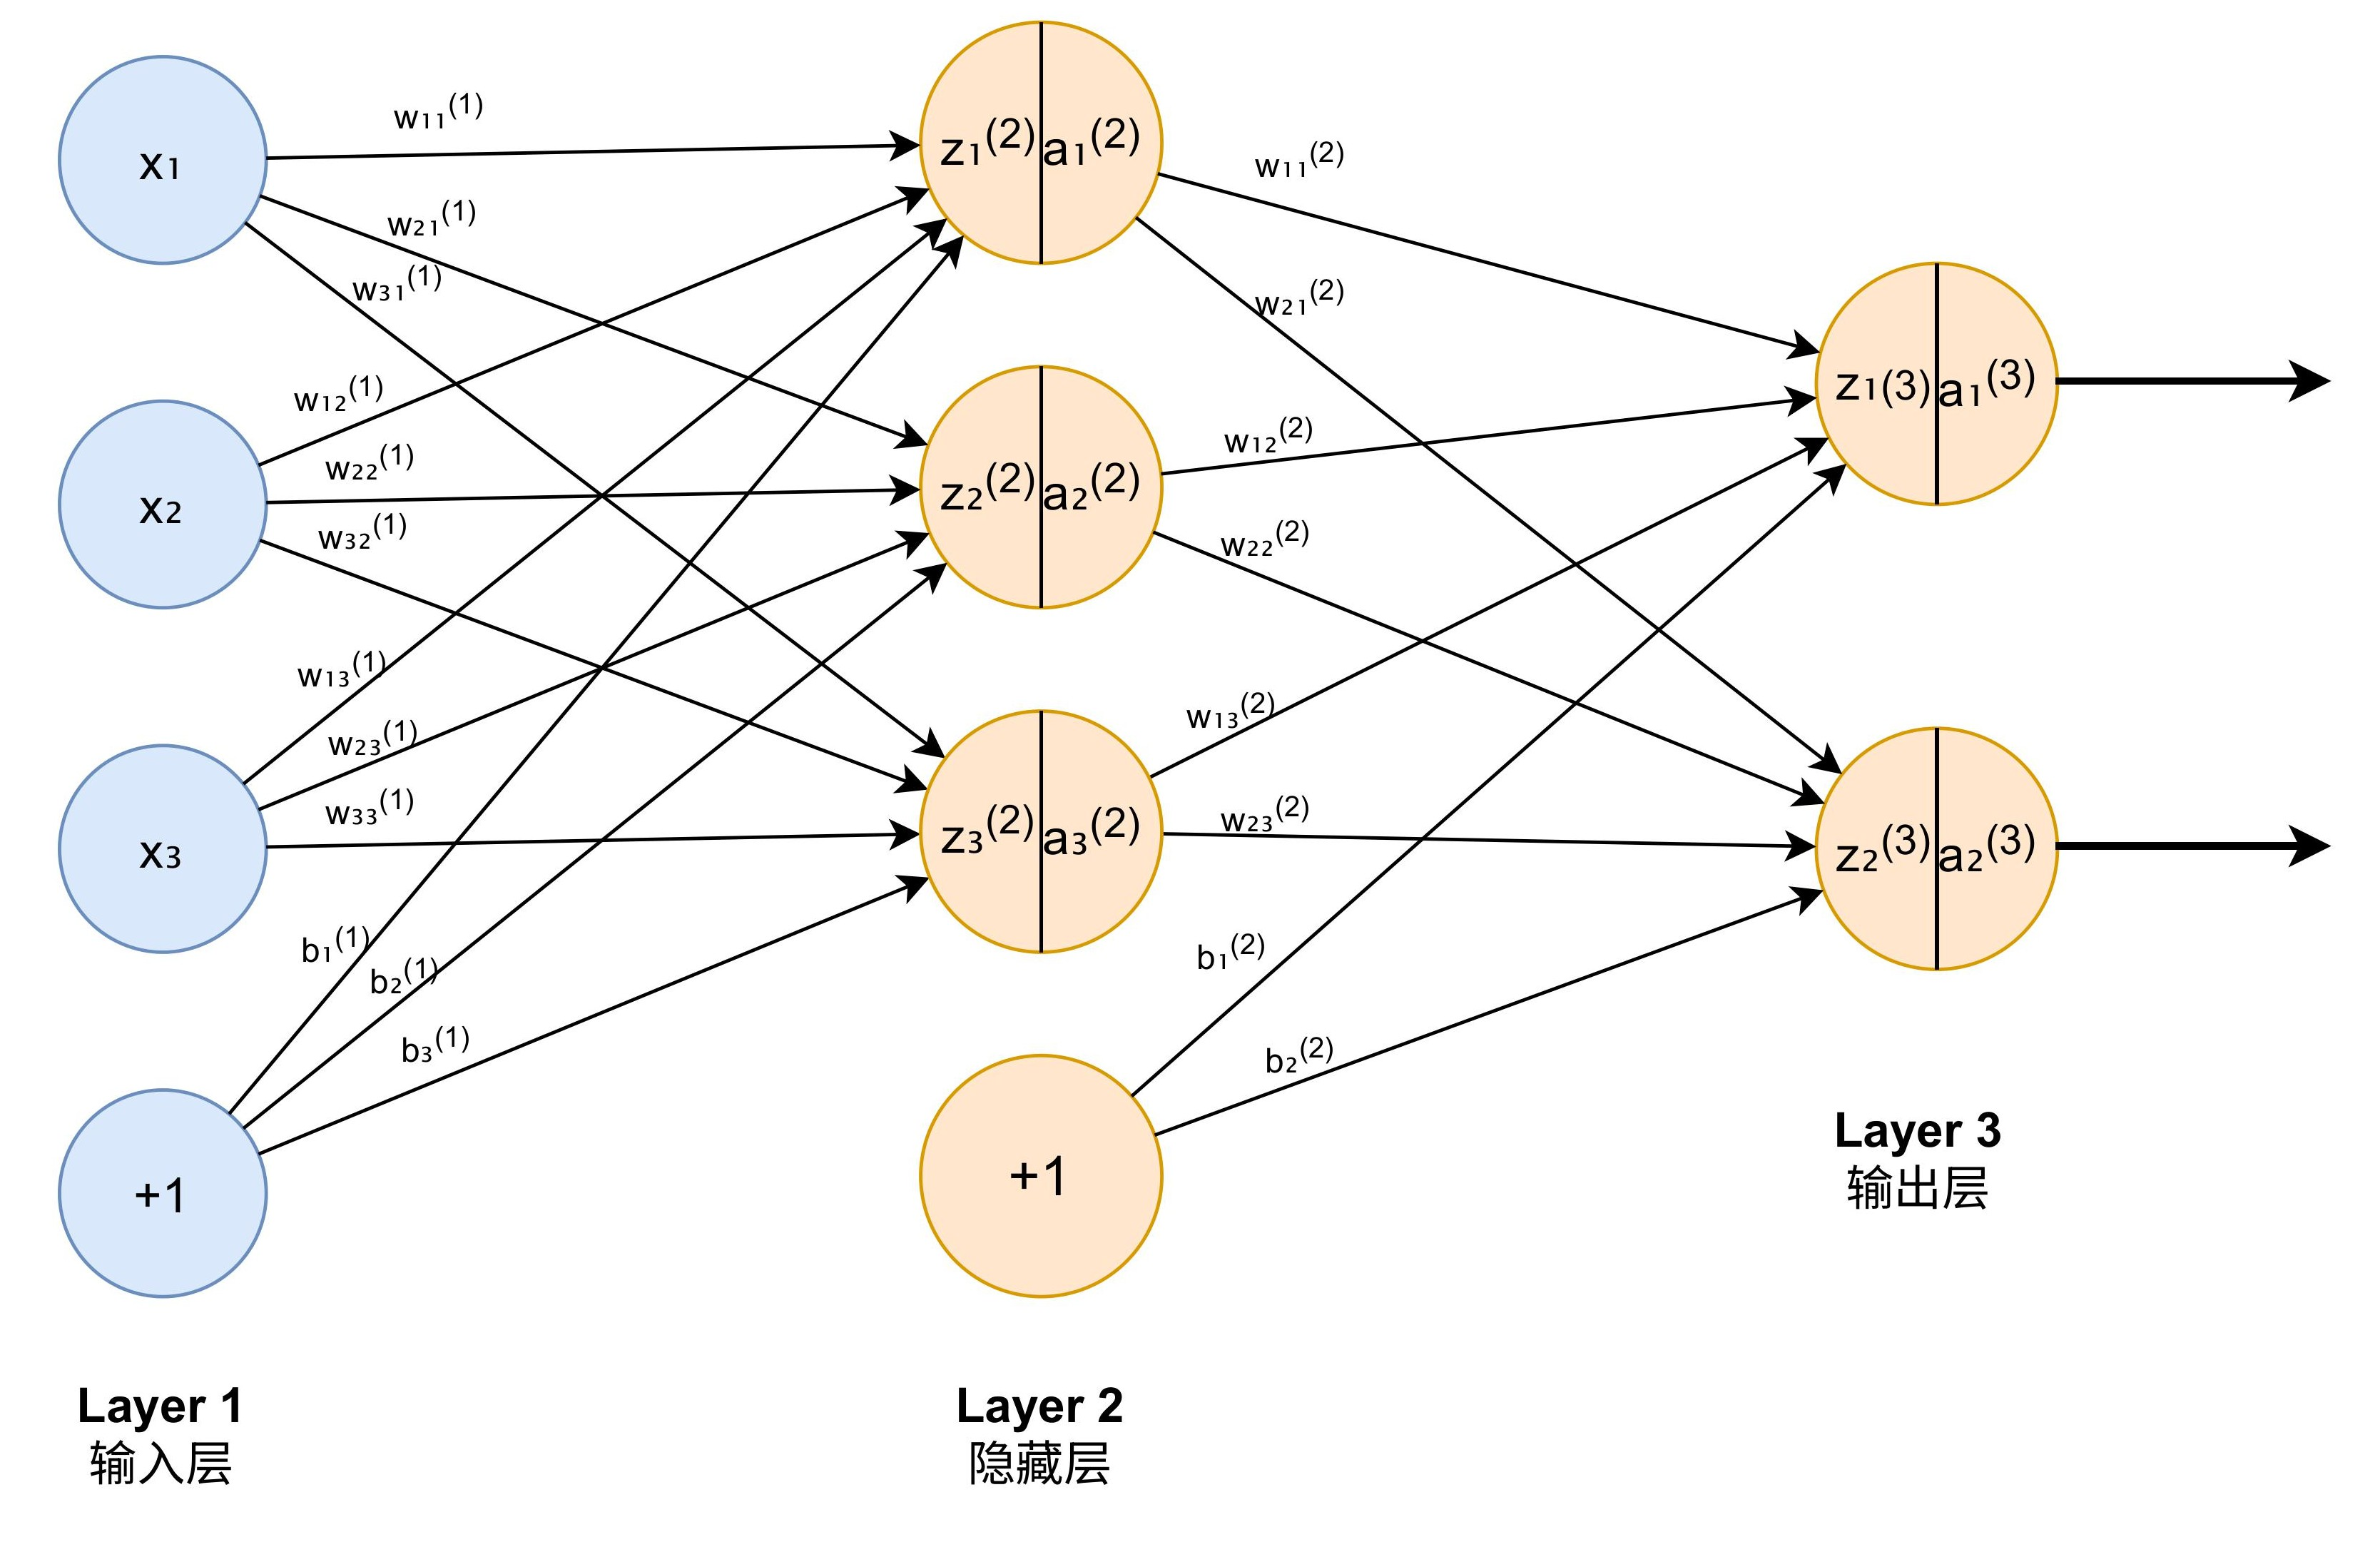
\includegraphics[width=\linewidth]{assets/04-deep-learning-1-01-neural-network.jpg}
\captionof{figure}{图 1：神经网络示意图，其中有竖线的@@橙色圆圈@@代表 neurons，@@有向边@@代表 params}

\textbf{紧凑形式}：

MLP 整体可视为一个复合函数： \[
  h(\mathbf{x}; \Theta) = \left( g_L \circ \tau_L \circ g_{L-1} \circ \tau_{L-1} \circ \cdots \circ g_1 \circ \tau_1 \right)(\mathbf{x})
\]

其中
\(\tau_\ell(\mathbf{a}) = \mathbf{W}^{(\ell)} \mathbf{a} + \mathbf{b}^{(\ell)}\)
为仿射变换，\(\circ\) 表示函数复合。

参数集合： \[
  \Theta =
  \left\{ \mathbf{W}^{(1)}, \mathbf{b}^{(1)}, \mathbf{W}^{(2)}, \mathbf{b}^{(2)},
  \ldots, \mathbf{W}^{(L)}, \mathbf{b}^{(L)} \right\}
\]

\textbf{激活函数}：

\begin{enumerate}
  \def\labelenumi{\arabic{enumi}.}
  \item
        \textbf{Sigmoid}：


        \centering
        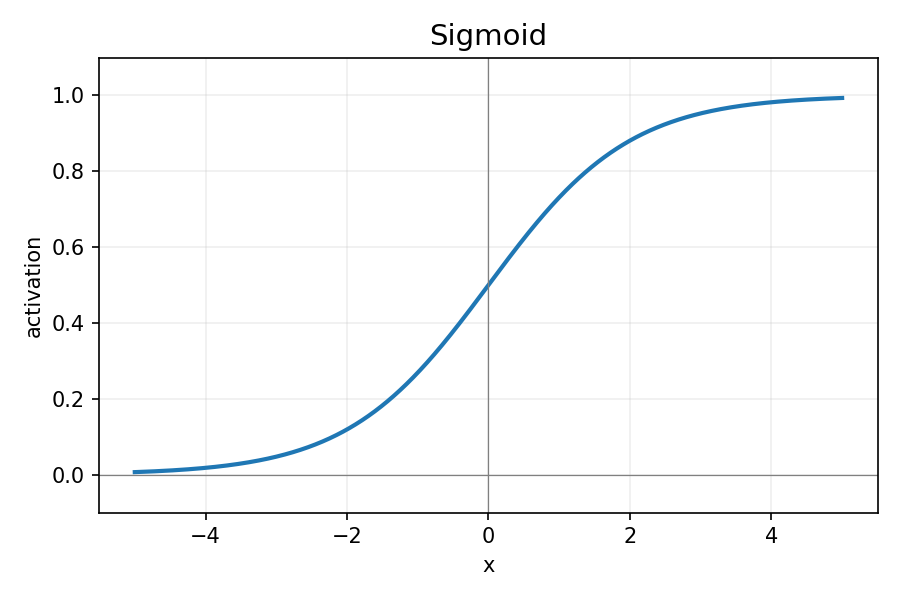
\includegraphics[width=\linewidth]{assets/04-deep-learning-1-02-sigmoid.png}
        \captionof{figure}{图 2：Sigmoid 函数}

        \[
          \sigma(x)=\frac{1}{1+e^{-x}},\quad \sigma'(x)=\sigma(x)(1-\sigma(x))
        \]

        \begin{itemize}
          \tightlist
          \item
                优点：概率化输出。\\
          \item
                缺点：易饱和导致梯度消失，输出非零中心。\\
          \item
                何时用：二分类输出层，隐藏层一般不推荐。
        \end{itemize}
  \item
        \textbf{tanh}：

        \centering
        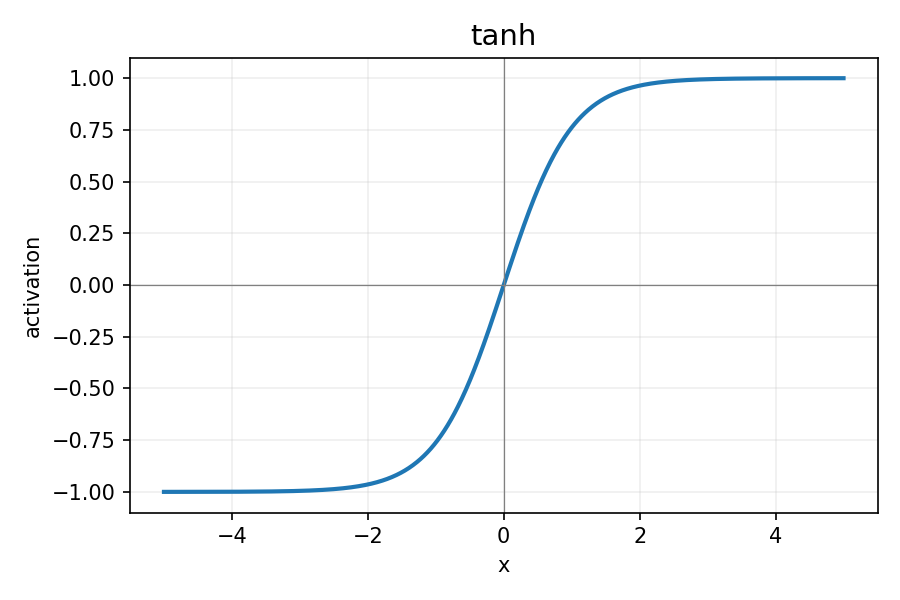
\includegraphics[width=\linewidth]{assets/04-deep-learning-1-03-tanh.png}
        \captionof{figure}{图 3：tanh 函数}

        \[
          \tanh(x)=\frac{e^x-e^{-x}}{e^x+e^{-x}},\quad \tanh'(x)=1-\tanh^2(x)
        \]

        \begin{itemize}
          \tightlist
          \item
                优点：输出以 0 为中心，训练通常比 sigmoid 稳定。\\
          \item
                缺点：仍会饱和（梯度消失）。\\
          \item
                何时用：历史上隐藏层曾常用，现代深层网络多用 ReLU。
        \end{itemize}
  \item
        \textbf{ReLU}：

        \centering
        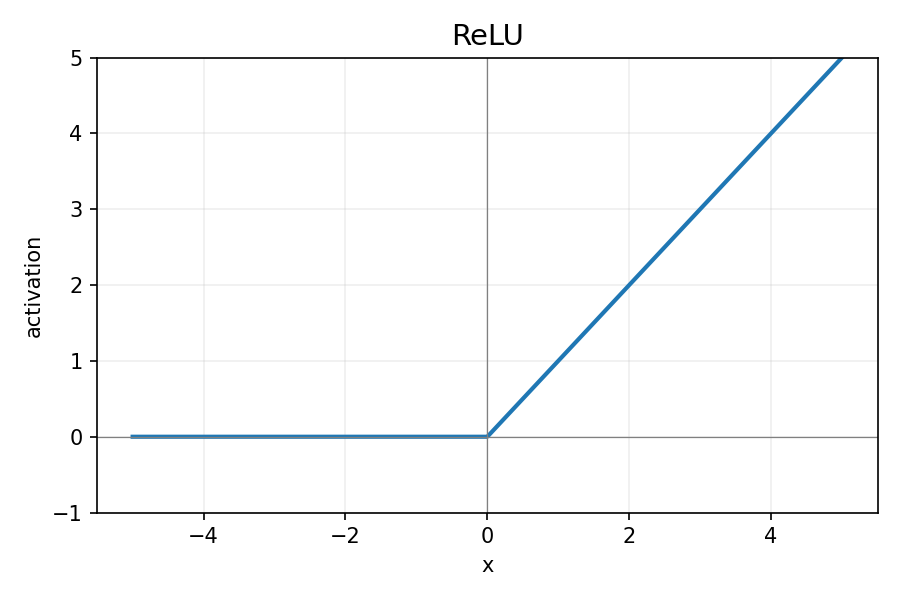
\includegraphics[width=\linewidth]{assets/04-deep-learning-1-04-relu.png}
        \captionof{figure}{图 4：ReLU 函数}

        \[
          \mathrm{ReLU}(x)=\max(0,x)
        \]

        \begin{itemize}
          \tightlist
          \item
                优点：计算简单、正区间梯度恒为
                1，缓解梯度消失，训练快且产生稀疏激活。\\
          \item
                缺点：可能出现 Dead ReLU（神经元输出恒为 0）。\\
          \item
                何时用：默认隐藏层首选激活。
        \end{itemize}
  \item
        \textbf{Leaky ReLU}：

        \centering
        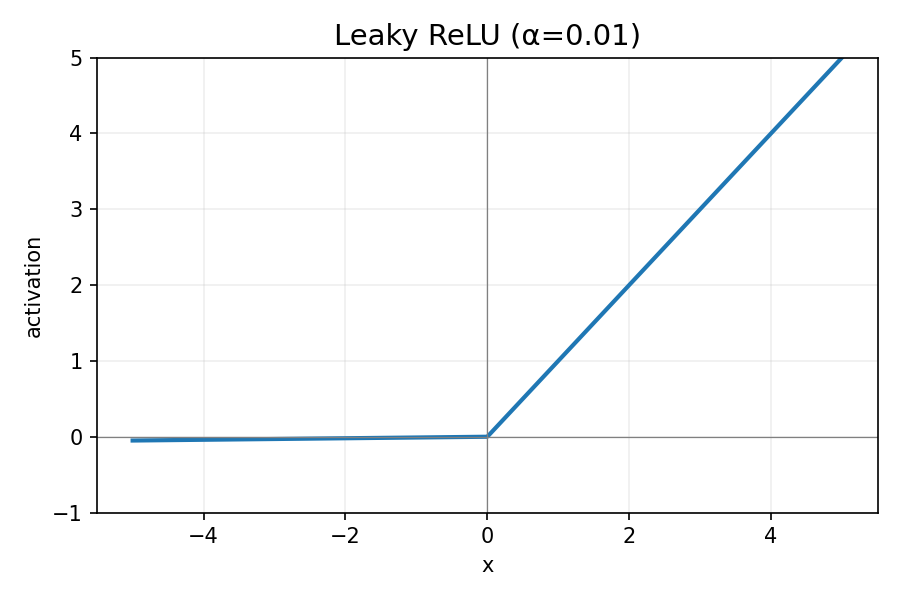
\includegraphics[width=\linewidth]{assets/04-deep-learning-1-05-leaky-relu.png}
        \captionof{figure}{图 5：Leaky ReLU 函数}

        \[
          \mathrm{LeakyReLU}(x)=\max(\alpha x,\,x)\quad(\text{usually }\alpha=0.01)
        \]

        \begin{itemize}
          \tightlist
          \item
                优点：较少死神经元，训练更稳健。\\
          \item
                缺点：引入小负输出，微弱影响稀疏性。\\
          \item
                何时用：遇到 Dead ReLU 或需更鲁棒时。
        \end{itemize}
  \item
        \textbf{ELU}：

        \centering
        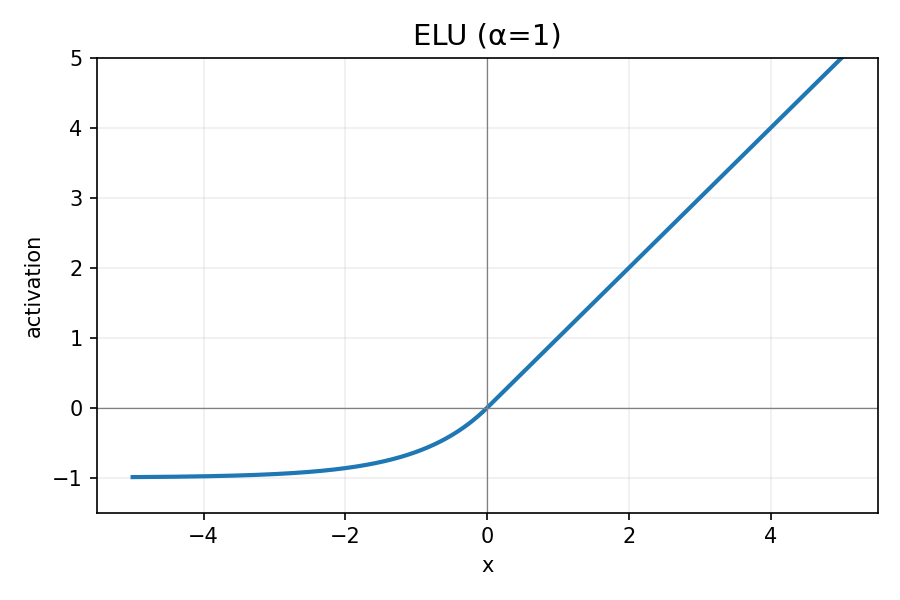
\includegraphics[width=\linewidth]{assets/04-deep-learning-1-06-elu.png}
        \captionof{figure}{图 6：ELU 函数}

        \[
          \mathrm{ELU}(x)=\begin{cases}x,&x\ge0,\\[4pt]\alpha(e^{x}-1),&x<0\end{cases}
        \]

        \begin{itemize}
          \tightlist
          \item
                优点：负区间平滑、均值可接近 0，训练稳定性好。\\
          \item
                缺点：含指数计算，开销比 ReLU 大。\\
          \item
                何时用：重视稳定性且能接受稍高计算成本时。
        \end{itemize}
  \item
        \textbf{Maxout}：

        \centering
        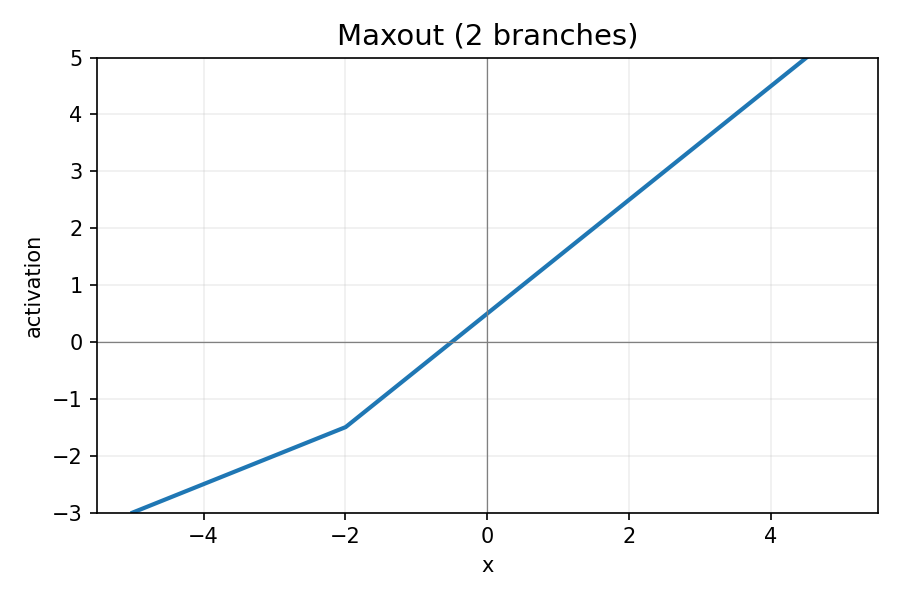
\includegraphics[width=\linewidth]{assets/04-deep-learning-1-07-maxout.png}
        \captionof{figure}{图 7：Maxout 函数}
        \[
          \mathrm{Maxout}(x)=\max(w_1^\top x+b_1,\; w_2^\top x+b_2)
        \]

        \begin{itemize}
          \tightlist
          \item
                优点：分段线性拟合能力强，对 Dropout 友好。\\
          \item
                缺点：参数与计算量成倍增加。\\
          \item
                何时用：需要更高模型容量且资源充足时。
        \end{itemize}
\end{enumerate}

\textbf{注}：ReLU 计算简单、正区间梯度为
1，可缓解梯度消失并加速收敛，是稳健的默认选择。

\subsubsection{Define the Loss Function}\label{define-the-loss-function}

我们要给出具体的损失函数与训练目标（optimization objective）。

\paragraph{MLE}\label{mle}

最大似然估计（Maximum Likelihood Estimation）。

把模型看作给定输入时产生输出标签的概率模型： \[
  p(y=1|x;\theta)=h(x; \theta),\quad p(y=0|x;\theta)=1-h(x; \theta).
\]

假设样本独立，则对整个训练集出现的概率估计（似然函数）为： \[
  p(Y|X;\theta)=\prod_{i=1}^n h(x^{(i)}; \theta)^{y^{(i)}} (1-h(x^{(i)}; \theta))^{1-y^{(i)}}.
\] 其中 \(Y\) 为标签向量，\(X\) 为输入向量，\(y^{(i)}\) 为第 \(i\)
个样本的标签，\(x^{(i)}\) 为第 \(i\) 个样本的输入。

每个模型（参数）都可以计算出对应的训练集似然。我们应当选取一个模型（参数），使得这个模型（参数）计算出的训练集似然是在整个模型空间（参数空间）中最大的。此即最大似然估计：
\[
  \theta^* = \arg\max_\theta p(Y|X;\theta)
\]

\paragraph{NLL/Cross-Entropy}\label{nllcross-entropy}

最大化似然等同于最小化负对数似然（Negative Log-Likelihood）。

\textbf{交叉熵}：

对于定义在同一个离散集合 $ \mathcal{X} $ 上的两个概率分布 $ P $ 和
$ Q $ \[
  H(P, Q) = -\sum_{x \in \mathcal{X}} P(x) \log Q(x)
\]

其中 \(H(\cdot,\ \cdot)\) 即为交叉熵函数。

\textbf{NLL/CE}：

针对这个二分类问题，为了使得梯度大小与样本数无关，我们取\textbf{平均形式}：
\[
  \begin{aligned}
    \mathcal{L}(\theta)
     & = -\frac{1}{n} \log p(Y|X;\theta)                                                                                 \\
     & = -\frac{1}{n} \sum_{i=1}^n \left[ y^{(i)}\log h(x^{(i)}; \theta) + (1-y^{(i)})\log(1-h(x^{(i)}; \theta)) \right] \\
     & = \frac{1}{n} \sum_{i=1}^n H(y^{(i)}, h^{(i)})
  \end{aligned}
\]

对单样本的损失： \[
  \begin{aligned}
    \ell^{(i)}(\theta)
     & = -\left[ y^{(i)}\log h(x^{(i)}; \theta) + (1-y^{(i)})\log(1-h(x^{(i)}; \theta)) \right] \\
     & = H(y^{(i)}, h^{(i)})
  \end{aligned}
\] 若加入 L2 正则化： \[
  \mathcal{L}_{\text{reg}}(\theta) = \mathcal{L}(\theta) + \frac{\lambda}{2}\|\theta\|^2
\] 其中 \(\lambda\) 为超参数。

\textbf{注}：

\begin{itemize}
  \tightlist
  \item
        NLL 使用对数，在概率极小时数值仍然稳定，且对于小概率惩罚更大。
  \item
        NLL 使用对数，将复杂乘法转化为加法。
  \item
        多元 NLL 和多元 CE 在数学上等价，不过 NLL 属于统计学，CE
        属于信息论（damn）
\end{itemize}

\subsubsection{Perform Fitting}\label{perform-fitting}

训练等价于最小化损失函数。我们分别推导 Logistic Regression 和 MLP
的反向传播过程。

\paragraph{Logistic Gradient Descent}\label{logistic-gradient-descent}

设 Logistic Regression 模型为：

\begin{itemize}
  \tightlist
  \item
        线性项 \(z = \theta^\top x\)
  \item
        输出 \(h = \sigma(z) = 1/(1+e^{-z})\)
  \item
        单样本损失 \(\ell(\theta) = -[ y\log h + (1-y)\log(1-h) ]\)
\end{itemize}

\textbf{链式法则求导}：

\begin{enumerate}
  \def\labelenumi{\arabic{enumi}.}
  \tightlist
  \item
        对 \(h\) 求导： \[
          \frac{\partial \ell}{\partial h} = -\left(\frac{y}{h} - \frac{1-y}{1-h}\right)
        \]
  \item
        对 \(z\) 求导： \[
          \frac{\partial h}{\partial z} = h(1 - h)
        \] 从而： \[
          \frac{\partial \ell}{\partial z}
          = \frac{\partial \ell}{\partial h} \frac{\partial h}{\partial z}
          = h - y
        \]
  \item
        对 \(\theta\) 求导： \[
          \frac{\partial \ell}{\partial \theta}
          = \frac{\partial \ell}{\partial z} \frac{\partial z}{\partial \theta}
          = (h - y) x
        \]
\end{enumerate}

\textbf{全量梯度}： \[
  \begin{aligned}
    \nabla_\theta \mathcal{L}(\theta)
     & = \frac{1}{n} \sum_{i=1}^n (h(x^{(i)}; \theta) - y^{(i)}) x^{(i)} \\
     & = \frac{1}{n} X^T (H - Y)
  \end{aligned}
\]

\textbf{注}：

\(h(x^{(i)}; \theta) - y^{(i)}\)
是模型的\textbf{预测误差}（残差），乘以输入 \(x^{(i)}\)
得到该样本对梯度的贡献。
误差的绝对值越大，说明在该样本上的预测越差，该样本对参数更新的影响越大，从而引导模型向减小该误差的方向调整。

\paragraph{MLP Backpropagation}\label{mlp-backpropagation}

对于多层神经网络，我们需要计算损失函数对每一层参数的梯度。反向传播算法通过链式法则高效地完成这一计算。

前向传播过程中有： \[
  \begin{aligned}
    \mathbf{z}^{(\ell)} & = \mathbf{W}^{(\ell)} \mathbf{a}^{(\ell-1)} + \mathbf{b}^{(\ell)} \\
    \mathbf{a}^{(\ell)} & = g_\ell(\mathbf{z}^{(\ell)})
  \end{aligned}
\]

其中
\(\mathbf{a}^{(1)} = \mathbf{x}\)，\(\mathbf{a}^{(L)} = h(\mathbf{x}; \Theta)\)
为最终输出。

定义\textbf{误差信号}： \[
  \boldsymbol{\delta}^{(\ell)} = \frac{\partial \mathcal{L}}{\partial \mathbf{z}^{(\ell)}}
\] 表示损失函数对第 \(\ell\) 层线性输出 \(\mathbf{z}^{(\ell)}\) 的梯度。

\begin{enumerate}
  \def\labelenumi{\arabic{enumi}.}
  \item
        \textbf{输出层误差}：

        对于二分类问题，输出层使用 Sigmoid 激活
        \(g_L(z) = \sigma(z)\)，损失为二元交叉熵：

        \[
          \boldsymbol{\delta}^{(L)} = \mathbf{a}^{(L)} - \mathbf{y}
        \]

        其中 \(\mathbf{y}\) 是标签向量。

        \textbf{证明}：以一维为例。 \[
          \begin{aligned}
            \delta^{(L)} & = \frac{\partial \mathcal{L}}{\partial z^{(L)}}
            = \frac{\partial \mathcal{L}}{\partial a^{(L)}} \cdot \frac{\partial a^{(L)}}{\partial z^{(L)}}   \\
                         & = \left(-\frac{y}{a^{(L)}} + \frac{1-y}{1-a^{(L)}}\right) \cdot a^{(L)}(1-a^{(L)}) \\
                         & = a^{(L)} - y
          \end{aligned}
        \]
  \item
        \textbf{误差反向传播}：

        对于隐藏层 \(\ell = L-1, L-2, \ldots, 2\)：

        \[
          \boldsymbol{\delta}^{(\ell)} = \left( (\mathbf{W}^{(\ell+1)})^\top \boldsymbol{\delta}^{(\ell+1)} \right) \odot g_\ell'(\mathbf{z}^{(\ell)})
        \]

        其中 \(\odot\) 表示逐元素相乘，\(g_\ell'\) 为激活函数的导数。

        \textbf{证明}： 根据链式法则，第 \(\ell\) 层的误差信号来自第
        \(\ell+1\) 层： \[
          \delta^{(\ell)}_j = \frac{\partial \mathcal{L}}{\partial z^{(\ell)}_j}
          = \sum_{k=1}^{n_{\ell+1}} \frac{\partial \mathcal{L}}{\partial z^{(\ell+1)}_k}
          \cdot \frac{\partial z^{(\ell+1)}_k}{\partial z^{(\ell)}_j}
        \]

        由于
        \(z^{(\ell+1)}_k = \sum_i w^{(\ell+1)}_{ki} a^{(\ell)}_i + b^{(\ell+1)}_k\)
        且 \(a^{(\ell)}_i = g_\ell(z^{(\ell)}_i)\)： \[
          \frac{\partial z^{(\ell+1)}_k}{\partial z^{(\ell)}_j} = w^{(\ell+1)}_{kj} \cdot g_\ell'(z^{(\ell)}_j)
        \]

        代入得： \[
          \delta^{(\ell)}_j = \left( \sum_{k} w^{(\ell+1)}_{kj} \delta^{(\ell+1)}_k \right) g_\ell'(z^{(\ell)}_j)
        \]

        写成矩阵形式即证。
  \item
        \textbf{权重梯度}：

        \[
          \frac{\partial \mathcal{L}}{\partial \mathbf{W}^{(\ell)}} = \boldsymbol{\delta}^{(\ell)} (\mathbf{a}^{(\ell-1)})^\top
        \]

        即： \[
          \frac{\partial \mathcal{L}}{\partial w^{(\ell)}_{ij}} = \delta^{(\ell)}_i \cdot a^{(\ell-1)}_j
        \]
  \item
        \textbf{偏置梯度}：

        \[
          \frac{\partial \mathcal{L}}{\partial \mathbf{b}^{(\ell)}} = \boldsymbol{\delta}^{(\ell)}
        \]
\end{enumerate}

\paragraph{Parameter Update Methods}\label{parameter-update-methods}

得到梯度后，使用优化器更新参数。

\begin{enumerate}
  \def\labelenumi{\arabic{enumi}.}
  \item
        全量批量梯度下降（\textbf{Full-batch GD}）：

        \[
          \theta' = \theta - \alpha \nabla_\theta \mathcal{L}(\theta)
        \]

        \begin{itemize}
          \tightlist
          \item
                优点：稳定。
          \item
                缺点：每步计算量大，不能很好地并行和进行实时更新。
        \end{itemize}
  \item
        随机梯度下降（Stochastic GD，\textbf{SGD}）：

        每次取一个样本更新： \[
          \theta' = \theta - \alpha (h_\theta(x^{(i)}) - y^{(i)}) x^{(i)}
        \]

        \begin{itemize}
          \tightlist
          \item
                优点：更新频繁、噪声可帮助跳出鞍点。
          \item
                缺点：噪声导致收敛震荡，不稳定。
        \end{itemize}
  \item
        小批量梯度下降（\textbf{Mini-batch GD}）：

        取 batch 为 \(\mathcal{B}\)，size 为 \(B\)： \[
          \theta' = \theta - \alpha \frac{1}{B}\sum_{i\in\mathcal{B}}(h_\theta(x^{(i)})-y^{(i)}) x^{(i)}
        \]

        在 GPU 上常用，平衡效率与稳定性。
  \item
        自适应优化器（\textbf{Adaptive Optimizers}）：

        \begin{itemize}
          \tightlist
          \item
                动量法：Momentum
          \item
                自适应学习率：Adam、RMSProp 等
        \end{itemize}
\end{enumerate}

\paragraph{Learning Rate}\label{learning-rate}

学习率 \(\alpha\) 的选择对训练很关键。

\textbf{常用策略}：

\begin{itemize}
  \tightlist
  \item
        固定学习率
  \item
        学习率衰减：

        \begin{itemize}
          \tightlist
          \item
                step decay：每隔若干 epoch 乘以一个衰减因子
          \item
                exponential decay：每轮指数衰减
        \end{itemize}
  \item
        基于验证集自动调整：
        监控验证集表现，若连续若干轮不提升，自动降低学习率。如 PyTorch 的
        \texttt{ReduceLROnPlateau}
  \item
        学习率预热： 训练初期用小学习率 warm up，逐渐增加到目标值，再衰减。
  \item
        提前停止： 监控验证集误差，若连续若干轮不下降则停止训练，防止过拟合。
\end{itemize}

\paragraph{Difficulty}\label{difficulty}

神经网络训练是\textbf{非凸}优化，常见问题：

\begin{itemize}
  \tightlist
  \item
        鞍点（saddle points）导致局部最优解。
  \item
        过参数化导致高维空间，其中有大量平坦区域（flat
        plateaus），梯度太小，移动慢；同时高维下特征值多，更容易出现鞍点（Hessian
        中正负特征值同时出现）。
\end{itemize}

因此，直接基于全量批量 GD 在深度学习中往往不够鲁棒，SGD
的噪声反而有帮助。

\subsubsection{Testing}\label{testing}

训练完成后要在\textbf{测试集}上评估模型的泛化能力（generalization）。

\textbf{Evaluation Metrics}：

缩写 \textbar{} 全称 \textbar{} 含义 \textbar{}\\
:--- \textbar{} :--- \textbar{} :--- \textbar{}\\
\textbf{TP} \textbar{} True Positives \textbar{} 1 预测为 1 的数量
\textbar{}\\
\textbf{FP} \textbar{} False Positives \textbar{} 0 预测为 1 的数量
\textbar{}\\
\textbf{FN} \textbar{} False Negatives \textbar{} 1 预测为 0 的数量
\textbar{}\\
\textbf{TN} \textbar{} True Negatives \textbar{} 0 预测为 0 的数量
\textbar{}

\begin{itemize}
  \tightlist
  \item
        准确率： \[
          \text{Accuracy} = \dfrac{\text{TP}+\text{TN}}{\text{TOT}}
        \]
  \item
        精确率： \[
          \text{Precision} = \dfrac{\text{TP}}{\text{TP}+\text{FP}}
        \]
  \item
        召回率： \[
          \text{Recall} = \dfrac{\text{TP}}{\text{TP}+\text{FN}}
        \]
  \item
        F1-score： \[
          2\dfrac{\text{Precision}\cdot\text{Recall}}{\text{Precision}+\text{Recall}}
        \]
  \item
        混淆矩阵（Confusion Matrix）：展示 TP/FP/TN/FN 的分布
  \item
        泛化间隙（Generalization Gap）： \[
          \text{Generalization Gap} = \mathbb{E}_{\text{test}}[\text{loss}] - \mathbb{E}_{\text{train}}[\text{loss}]
        \]
\end{itemize}

\centering
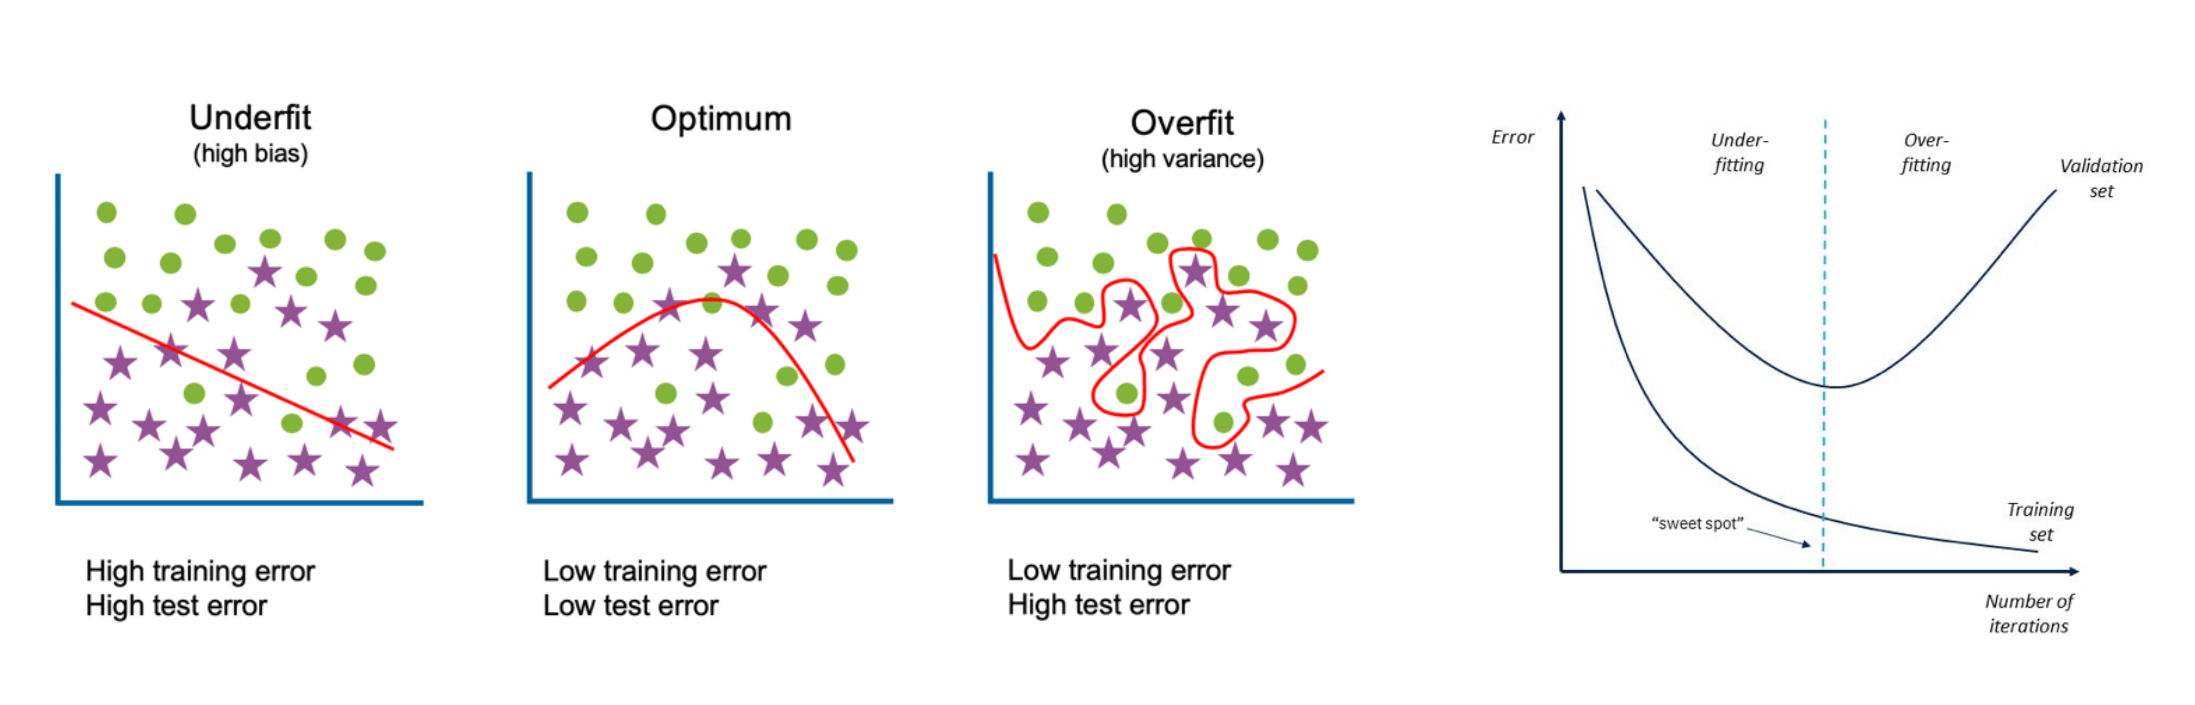
\includegraphics[width=\linewidth]{assets/04-deep-learning-1-08-underfitting-and-overfitting.png}
\captionof{figure}{图 8：欠拟合与过拟合图示}

\textbf{注}：

\begin{itemize}
  \item
        Loss 降低不代表 Accuracy 升高。例如：

        \textbar{} 样本 \textbar{} 训练前预测 (\(p_1\), \(p_2\)) \textbar{}
        结果 \textbar{} 训练后预测 (\(p_1\), \(p_2\)) \textbar{} 结果
        \textbar{} \textbar{} ---- \textbar{} ------------------- \textbar{}
        ---- \textbar{} ----------------- \textbar{} ---- \textbar{}
        \textbar{} A \textbar{} (0.51, 0.49) \textbar{} 正确 \textbar{} (0.99,
        0.01) \textbar{} 正确 \textbar{} \textbar{} B \textbar{} (0.51, 0.49)
        \textbar{} 正确 \textbar{} (0.49, 0.51) \textbar{} 错误 \textbar{}

        \textbar{} 指标 \textbar{} 训练前 \textbar{} 训练后 \textbar{}
        \textbar{} ---- \textbar{} ------ \textbar{} ----- \textbar{}
        \textbar{} Accuracy \textbar{} 100\% \textbar{} 50\% \textbar{}
        \textbar{} Loss \textbar{} 更高 \textbar{} 更低 \textbar{}
\end{itemize}

\begin{center}\rule{0.5\linewidth}{0.5pt}\end{center}

\subsection{Problems for Applying MLP to
  CV}\label{problems-for-applying-mlp-to-cv}

需要将图像平坦化（flatten）为向量：

\begin{itemize}
  \tightlist
  \item
        会破坏图像的局部结构，\textbf{空间邻接}关系在展平的向量中不再邻接。
  \item
        参数数目随像素数线性增长，对高分辨率图像\textbf{计算与内存负担大}。
  \item
        对于输入图像的微小平移操作，MLP
        很难保持输出基本不变，也即\textbf{很难具有平移不变性}。
\end{itemize}

因此在视觉任务中更常用 \textbf{Convolutional Neural
  Networks（CNNs）}，保留空间结构并通过参数共享大幅减少参数量。
